% ======================================================================
%  Kapitel: Auswertung  --  gekuerzte und korrigierte Fassung
%
%  Aenderungen gegenueber der Vorfassung:
%   - Faktor 1/2 in der besetzten Schranke ergaenzt (zweimal); Verweis
%     auf eq:gap-bound statt eq:bendavid-diff, Divergenz ueber den
%     Randverteilungen notiert -- vgl. korrigiertes Kapitel 3
%   - "Zuweisungsgrenze" durch "kritische Groesse" ersetzt
%   - "bitidentisch" bei FP16 auf "identische Metrikwerte" abgeschwaecht
%   - Precision-Argument in der Ablation und in der Fehleranalyse
%     auf den richtigen Nenner (Detektionszahl) bezogen
%   - SHA-256-Angabe als gekuerzt gekennzeichnet
%   - Inferenzparameter-Absatz, Zylindermodell-Erlaeuterung,
%     Schranken-Gegenprobe und die beiden Einschraenkungsabsaetze
%     der Ablation zusammengefuehrt und gekuerzt
%   - Ablation B (Herkunft der Okkluder) gestrichen; die Einbettung ist die
%     einzige Ablation
%
%  Mit "% PRUEFEN" markierte Stellen brauchen eine Entscheidung.
% ======================================================================

\chapter{Auswertung}
\label{kap:auswertung}

\section{Metriken und Bewertungsprotokoll}
\label{sec:metriken}

Eine Detektion gilt als Treffer, wenn ihre Box eine Ground-Truth-Box mit einer
\emph{Intersection over Union} nach Gleichung~\eqref{eq:ioudef} von mindestens
$t_{\IoU}$ überdeckt; jede Ground-Truth-Box kann höchstens einmal getroffen
werden. Daraus folgen
\emph{Precision} $P$, \emph{Recall} $R$ und deren harmonisches Mittel $F_1$;
berichtet wird stets das beste $F_1$ über alle Konfidenzschwellen samt der
zugehörigen Schwelle $c^*$. Diese Schwelle wird je Split nachträglich bestimmt,
für \code{test} also auf dem Testbild selbst; in einer Anwendung wäre sie wie
die Auflösung (Abschnitt~\ref{sec:imgsz}) auf \code{val} zu wählen. Die
$F_1$-Werte sind deshalb als obere Schranke des erreichbaren Betriebspunkts zu
lesen. \emph{mAP} ist die Fläche unter der Precision-Recall-Kurve
\parencite{everingham2010}; \mAPfifty{} verwendet $t_{\IoU} = 0{,}5$,
\mAPseven{} $t_{\IoU} = 0{,}75$ und \mAPall{} den Mittelwert über
$t_{\IoU} = 0{,}50; \dots; 0{,}95$ nach
COCO-Konvention \parencite{lin2014coco}. Leitgröße dieser Arbeit ist
\mAPfifty{}: Bei Objektdurchmessern um 20\px{} misst \mAPall{} zu einem
erheblichen Teil die Pixelauflösung und die Labelkonvention und nicht die
Detektionsgüte; Abschnitt~\ref{sec:boxversatz} weist das nach.

Die Bewertung erfolgt über eine eigene Implementierung, weil die mittlere
Treffer-IoU und der $F_1$-optimale Betriebspunkt gebraucht werden; diese
Größen gibt die Standardfunktion der Werkzeugkette nicht aus. Zur Absicherung
wurde sie gegen die Referenzimplementierung geprüft: \code{val}
\zxcValEigen/\zxcValEigenA{} gegen \zxcValUlt/\zxcValUltA{} und \code{test}
\zxcTestEigen/\zxcTestEigenA{} gegen \zxcTestUlt/\zxcTestUltA{}
(\mAPfifty{}/\mAPall{}). Die Abweichung von höchstens \zxcMaxDiff\,Prozentpunkten
geht vermutlich auf die Zuordnung zurück: Beide Implementierungen interpolieren
die AP über 101 Punkte, die Werkzeugkette ordnet Detektionen aber nach IoU statt
nach Konfidenz zu (\code{match\_predictions} in
\code{ultralytics/engine/validator.py}, Version~8.4.117).

Zwei Angaben gelten für alle folgenden Zahlen. \emph{Erstens} wird, wo nichts
anderes steht, beim \textbf{nativen Maßstab} ausgewertet: \code{imgsz} gleich
der längsten Bildkante, auf ein Vielfaches von 32 aufgerundet, also 2464 für
\code{val} (native Breite 2459\px) und 1600 für \code{test}. Das ist der
einzige Wert, der ohne eine Auswahlentscheidung feststeht; jede andere Wahl
müsste erst begründet werden und würde die Ablation von einer nachgelagerten
Optimierung abhängig machen. \emph{Zweitens} umfassen die Bewertungsdaten
98 (\code{val}) und 89 (\code{test}) Objekte (Abschnitt~\ref{sec:valtest}).

\section{Hauptergebnis und Sim-to-Real-Abstand}
\label{sec:hauptergebnis}

\begin{table}[htbp]
\centering
\caption[Hauptergebnis]{Ergebnis des Referenzmodells (\code{yolo26s-p2}, 6000 Bilder, 60 Epochen) bei nativem Maßstab. $c^*$ ist die $F_1$-optimale Konfidenzschwelle, $P$ und $R$ sind Precision und Rückruf an diesem Betriebspunkt.}
\label{tab:hauptergebnis}
\footnotesize
\begin{tabular}{@{}lrrrrrrr@{}}
\toprule
\textbf{Split} & \mAPfifty{} & \mAPseven{} & \mAPall{} & \textbf{bestes $F_1$} & $c^*$ & $P$\,/\,$R$ & \textbf{mittl.\ IoU} \\
\midrule
\code{val} (real) & \textbf{0{,}916} & 0{,}753 & 0{,}580 & 0{,}864 & 0{,}119 & 0{,}851\,/\,0{,}878 & 0{,}801 \\
\code{test} (real) & \textbf{0{,}955} & 0{,}382 & 0{,}478 & 0{,}925 & 0{,}266 & 0{,}952\,/\,0{,}899 & 0{,}752 \\
\code{sval} (synth.) & \textbf{0{,}984} & 0{,}952 & 0{,}830 & 0{,}962 & 0{,}419 & 0{,}967\,/\,0{,}957 & 0{,}900 \\
\bottomrule
\end{tabular}
\end{table}


Ein ausschließlich auf synthetischen Bildern trainiertes Modell erreicht auf
echten, nie im Training gesehenen Aufnahmen \mAPfifty{} von
\textbf{\zrefValMap} (\code{val}) und \textbf{\zrefTestMap} (\code{test}); das
ist die Antwort auf die Aufgabenstellung (Tabelle~\ref{tab:hauptergebnis}). Am
$F_1$-optimalen Betriebspunkt erreicht es einen Rückruf von \zrefValRec{}
(\code{val}) bzw.\ \zrefTestRec{} (\code{test}) bei einer Precision von
\zrefValPrec{} und \zrefTestPrec: Auf \code{test} liefert es \znPredTest{}
Detektionen, von denen nur \zfpTest{} falsch-positiv sind, \zfpDoppelTest{} davon
als zweite Box auf einer schon erkannten Stirnfläche, und übersieht \zfnTest{}
der 89 Stirnflächen.

Der auffällige Unterschied zwischen den Splits -- \mAPseven{} \zrefValMapS{}
auf \code{val}, aber nur \zrefTestMapS{} auf \code{test} bei \emph{höherem}
\mAPfifty{} -- ist kein Widerspruch. Ein Teil davon ist die in
Abschnitt~\ref{subsec:kleine-objekte} beschriebene Empfindlichkeit der IoU bei
kleinen Objekten: Die Objekte in \code{test} sind kleiner (gemessener Median
17,0 gegen 26,8\px, Tabelle~\ref{tab:statistik}), und die mittlere Treffer-IoU
bestätigt den Unterschied direkt (\zrefTestIou{} gegen \zrefValIou). Der
größere Teil ist ein \emph{systematischer Größenversatz zwischen
Generatorlabel und Handannotation}, der in Abschnitt~\ref{sec:boxversatz}
aufgeschlüsselt wird. \mAPall{} ist bei dieser Objektgröße daher weniger ein
Maß für die Detektionsqualität als für Pixelauflösung und Labelkonvention;
diese Feststellung gilt für alle folgenden Tabellen. Wo das Modell auf beiden
Realbildern richtig und wo es falsch detektiert, zeigt
Abbildung~\ref{abb:qualitativ} in
Abschnitt~\ref{sec:bootstrap}.

\absatz{Sim-to-Real-Abstand.}\label{sec:simtoreal}
Der Split \code{sval} besteht aus 400 synthetischen Bildern derselben Pipeline
mit anderem Seed. Mit ihm lassen sich zwei Fragen trennen: ob das Modell die
Aufgabe überhaupt lösen kann und ob sich das Gelernte auf echte Bilder
überträgt. Auf \code{sval} erreicht das Modell \zrefSvalMap{} \mAPfifty, auf
den realen Bildern liegt es um \zsimRealVal{} (\code{val}) bzw.\
\zsimRealTest\PP{} (\code{test}) darunter. Bei \mAPall{} ist der Abstand mit
\zsimRealValA{} bzw.\ \zsimRealTestA\PP{} viel größer.

Ein Teil dieses großen Abstands ist ein Messartefakt. \code{sval} ist mit
Generatorlabels beschriftet, die realen Bilder von Hand, und zwischen beiden
liegt der Größenversatz aus Abschnitt~\ref{sec:boxversatz}. Rechnet man ihn mit
der Sensitivitätsrechnung heraus (Tabelle~\ref{tab:boxsens} im Anhang), sinkt
der Abstand bei \mAPall{} auf \zsimRealTestAKorr{} (\code{test}) bzw.\
\zsimRealValAKorr\PP{} (\code{val}). Es bleibt also ein großer Rest, den diese
Arbeit nicht erklären kann. Belastbar sind deshalb nur die Aussagen über
\mAPfifty{} und den $F_1$-Betriebspunkt, auf die sich die Leitgröße aus
Abschnitt~\ref{sec:metriken} ohnehin beschränkt.

Bei \mAPfifty{} spielt der Größenversatz keine Rolle: Werden die Boxen
aufgeweitet, steigt \mAPfifty{} nicht, auf \code{test} sinkt es sogar leicht.
Der Abstand bei \mAPfifty{} geht also nicht auf die Boxgröße zurück. Andere
Unterschiede der Beschriftung kann er aber enthalten, etwa welche teilverdeckten
Enden überhaupt ein Label erhalten (Abschnitt~\ref{sec:sichtbarkeit}). Auf \code{test} zeigt er auch nicht das
Muster, das bei reinem Artefaktlernen zu erwarten wäre: Hätte das Netz eine der
Signaturen S1--S6 als Abkürzung gelernt, würde es auf \code{sval} zwar ähnliche
Werte erreichen, auf den realen Bildern aber deutlich niedrigere.

Wie groß der Abstand ist, ordnet zum einen die Ablation ein
(Abschnitt~\ref{sec:ablationC}), zum anderen die Stichprobenunsicherheit aus
Abschnitt~\ref{sec:bootstrap}. Auf \code{val} liegt der Wert \zrefSvalMap{}
von \code{sval} über dem 95\,\%-Intervall $[\zbootValLo;\,\zbootValHi]$. Dort
ist der Abstand also größer als die Messunsicherheit, und nach
Abschnitt~\ref{sec:sim2real} zeigt er, dass sich die Domänen unterscheiden,
aber nicht, ob in den Bildern oder in den Beschriftungen. Auf \code{test} liegt
derselbe Wert dagegen noch im Intervall $[\zbootTestLo;\,\zbootTestHi]$; der
Abstand beträgt dort \zsimRealTest\PP{} und ist von der Messunsicherheit nicht
zu unterscheiden. Nach Abschnitt~\ref{sec:sim2real} heißt das nicht, dass die
Domänen gleich sind, sondern nur, dass sich auf diesem Bild keine Wirkung
ihrer Unterschiede auf \mAPfifty{} nachweisen lässt. Die Unsicherheit von
\code{sval} selbst ist dabei nicht berücksichtigt; gemessen wurde sie nicht,
bei 400 Bildern dürfte sie aber deutlich kleiner sein als die eines einzelnen
Realbilds.

\section{Die Inferenzauflösung}
\label{sec:imgsz}

Die Inferenzauflösung ist der wirksamste Parameter, der nach dem Training noch
frei ist; ihr Wert wird gemessen und nicht begründet. Dafür wird kein Modell neu
trainiert. Dasselbe Modell wird bei neun Auflösungen zwischen 640 und
2464\px{} ausgewertet; unter ihnen ist für jeden Split auch der native Maßstab
(2464 für \code{val}, 1600 für \code{test}).


Von \code{imgsz}~640 auf \zswValBestAt{} steigt \mAPfifty{} auf \code{val} von
\zswValNiedrig{} auf \zswValBest. Mit \zswValGain\,Prozentpunkten ist das die
größte gemessene Spanne der Arbeit. Mit einer Ablationsdifferenz ist sie
allerdings nicht direkt vergleichbar, denn sie schließt eine bewusst ungünstige
Einstellung ein, und einzelne Entscheidungen der Augmentierungspipeline wurden
nicht abliert. Die Erklärung ist rein geometrisch und folgt aus
Abschnitt~\ref{subsec:kleine-objekte}: Nach Gleichung~\eqref{eq:deff} schrumpft
jedes Objekt mit dem Verhältnis $M/N$ aus Netzeingabe und Bildkantenlänge. Für
\code{val} ist $N = 2459$\px{} (Tabelle~\ref{tab:statistik}), bei $M = 640$ also
$M/N = 0{,}26$. Die 12--36\px{} großen Objekte kommen dann nur noch mit
3--9\px{} im Netz an, und der Rückruf bricht auf \zswValNiedrigRec{} ein. Das
Modell lokalisiert die Objekte also nicht nur ungenauer, sondern \emph{findet}
die meisten von ihnen nicht mehr. Auf \code{test} ist der Einbruch mit \zswTestGain\,Prozentpunkten kleiner,
weil das Bild nur 1600\px{} breit ist und deshalb weniger stark verkleinert
wird.

Der P2-Kopf verhindert diesen Einbruch nicht. Die kritische Größe $S\sqrt{2}$
aus Gleichung~\eqref{eq:gridmiss} sagt nur, ob ein Objekt überhaupt eine
Gitterposition erhält. Ein 5\px{} großes Objekt ist aber auch mit
Gitterposition kaum noch von einem dunklen Loch im Maschendraht zu
unterscheiden, und es liegt außerdem außerhalb der Trainingsverteilung, die nach
unten nur bis 7,2\px{} reicht (Abschnitt~\ref{sec:trainparam}).

\absatz{Das Optimum liegt dort, wo die Objektgröße zur Trainingsverteilung
passt.} Der Generator erzeugt Objekte mit Median 23,5\px{}
(Tabelle~\ref{tab:parameter}, T2), und in diesem Bereich liegt auch das Maximum
beider Kurven in Abbildung~\ref{abb:imgsz}. Auf \code{val} ist \mAPfifty{} bei
\code{imgsz}~\zswValBestAt{} und 2240 gleich hoch (\zswValBest); der gemessene
\code{val}-Median von 26,8\px{} kommt dort nach Gleichung~\eqref{eq:deff} mit
\zswValBestDeff{} bzw.\ 24,4\px{} im Netzeingang an. Auf \code{test} liegt das
Maximum bei \code{imgsz}~\zswTestBestAt{} (\zswTestBest) mit \zswTestBestDeff\px.
Beide Werte liegen nahe am Trainingsmedian, obwohl die beiden Bilder
unterschiedlich groß sind und unterschiedlich große Objekte enthalten.
Sichtbar ist der Effekt aber nur in einer Richtung. Eine zu \emph{kleine}
Auflösung wirkt sich stark aus (bei 960 kommt der \code{val}-Median mit
10,4\px{} an). Sobald der Median im Netzeingang etwa 17\px{} erreicht, auf
\code{val} ab 1600, auf \code{test} ab dem nativen Maßstab, ändert sich dagegen
wenig: Auf diesem Plateau bleiben die Unterschiede auf beiden Splits innerhalb
der Messunsicherheit aus Abschnitt~\ref{sec:bootstrap}, und auf \code{test}
liegt \mAPfifty{} selbst bei \zswTestHochAt{} mit \zswTestHoch{} kaum unter dem
Maximum.

Daraus folgt eine praktische Regel und eine methodische Feststellung. Die
Regel: die Auflösung so wählen, dass die erwartete Objektgröße im Netzeingang
im Bereich der Trainingsverteilung liegt und keinesfalls deutlich darunter; ob
ihr Median selbst das Optimum trifft, lässt sich bei dieser Messunsicherheit
nicht entscheiden. Die Feststellung: Objektgrößenbereich des Generators und
Inferenzauflösung sind \emph{nicht} unabhängig voneinander wählbar; eine
Entscheidung in der Datenerzeugung legt eine Entscheidung zur Inferenzzeit
fest.

Für den Einsatz wäre die Auflösung allein auf \code{val} zu wählen und
unverändert auf \code{test} zu übertragen, denn eine eigene Wahl für
\code{test} wäre eine Optimierung auf dem Testsatz; berichtet wird hier
dennoch beim nativen Maßstab (Abschnitt~\ref{sec:metriken}).

Die übrigen Inferenzparameter sind unkritisch: Der NMS-Schwellwert wirkt beim
Ende-zu-Ende-Modell nicht, weil keine NMS läuft (Abschnitt~\ref{sec:yolo26}).
Die Test-Time-Augmentation führt die Werkzeugkette bei diesem Modell nicht
aus, sie fällt mit einer Warnung auf die einfache Vorhersage zurück
(\code{\_predict\_augment} in \code{ultralytics/nn/tasks.py},
Version~8.4.117). Der Parameter \code{max\_det} verändert ab 100 den
Betriebspunkt und ab 200 auch \mAPfifty{} nicht mehr, und FP16 liefert
identische Metrikwerte (\code{src/experiment.py infer}).

\begin{figure}[htbp]
\centering
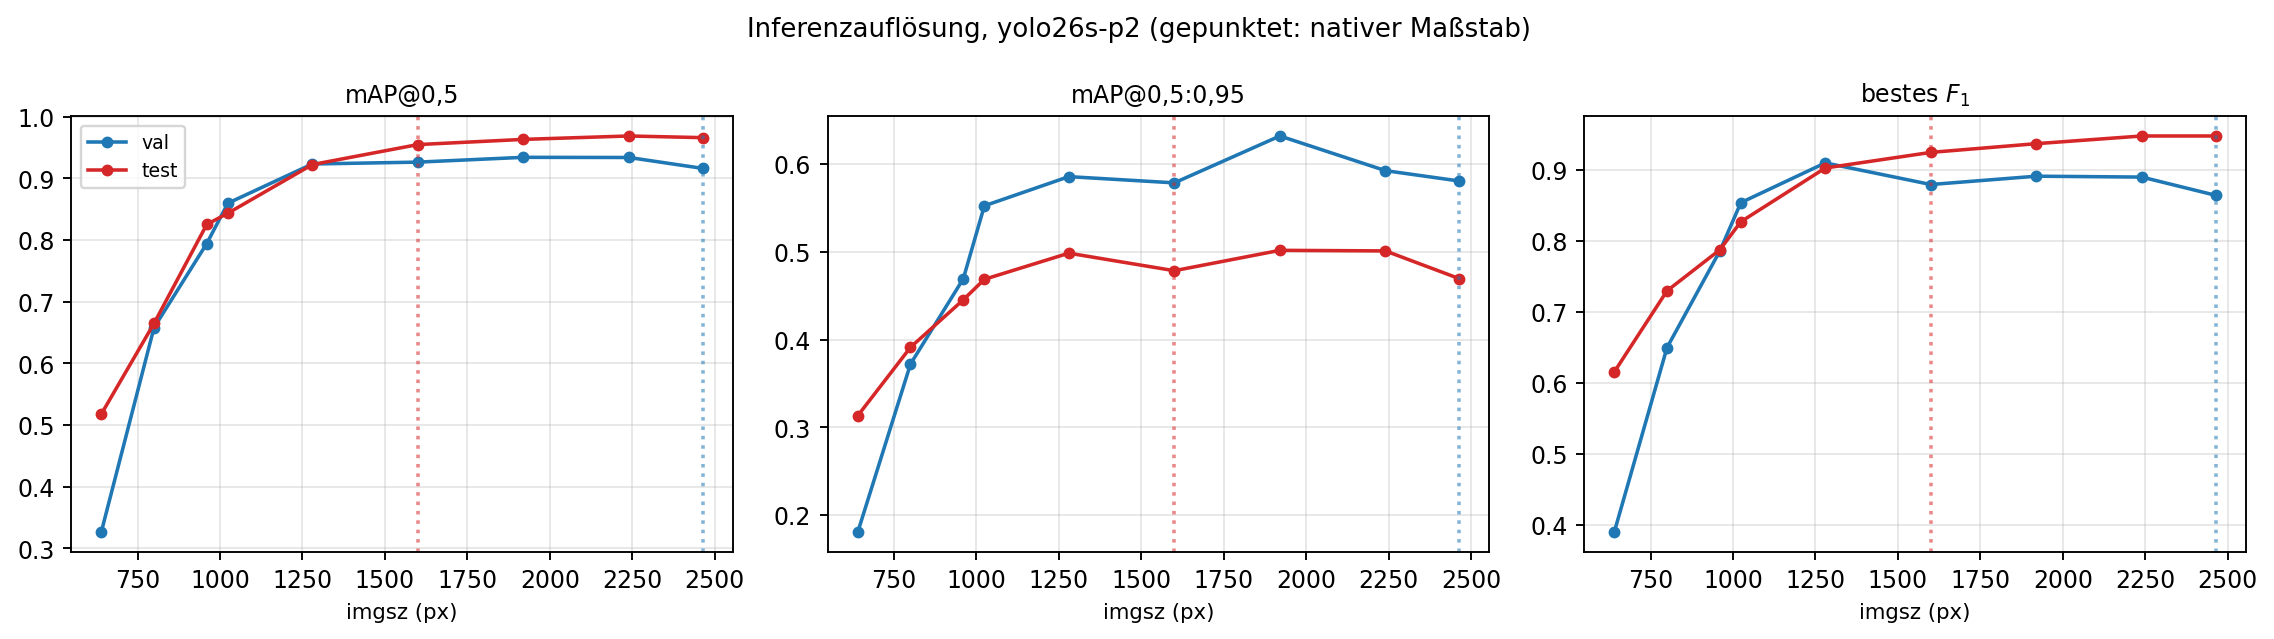
\includegraphics[width=\textwidth]{abbildungen/neu_imgsz.png}
\caption[Inferenzauflösung]{Metriken über die Inferenzauflösung für das
Referenzmodell \code{yolo26s-p2}; gepunktet der native Maßstab je Split. Der
Verlauf ist auf beiden Splits derselbe: steiler Anstieg, bis der Objektmedian im
Netzeingang etwa 17\px{} erreicht, danach ein flaches Optimum. Die Zahlen stehen vollständig in
Tabelle~\ref{tab:imgszvoll} im Anhang.}
\label{abb:imgsz}
\end{figure}

\section{Die Ablation: Wie viel trägt die Einbettung?}
\label{sec:ablationC}

\absatz{Motivation.} Die Ablation prüft keine einzelne Stufe, sondern
das Leitprinzip der Pipeline (Kapitel~\ref{kap:pipeline}), das das
Einfügen selbst betrifft. Jede Stufe, die gegen eine der Signaturen
S1--S6 gerichtet ist, kostet Rechenzeit und wird mit demselben Argument
begründet: Ein eingefügtes Objekt, das sich statistisch von seiner Umgebung
unterscheidet, könnte als Abkürzung dienen. Gestützt war dieses Argument bisher
nur \emph{indirekt} durch den Sim-to-Real-Abstand des Referenzmodells
(Abschnitt~\ref{sec:hauptergebnis}), also durch ein Indiz. Die Ablation prüft
es direkt, indem sie alle diese Maßnahmen zusammen abschaltet.

\absatz{Versuchsaufbau.} Zwei Arme, beide mit dem reduzierten Budget aus
Tabelle~\ref{tab:budgets} trainiert und deshalb nur untereinander vergleichbar
(\code{yolo26s-p2}, 3000~Bilder, 30~Epochen, Batch~8, Seed~0,
\code{imgsz}=1024, Auswahl über dasselbe reale \code{val}-Bild):

\begin{description}[leftmargin=1.4em,itemsep=2pt,font=\normalfont\bfseries]
  \item[C0 Kontrolle] die vollständige Pipeline aus
  Kapitel~\ref{kap:pipeline}, mit demselben Codestand erzeugt wie C1.
  \item[C1 naiv eingeklebt] dieselbe Pipeline mit abgeschalteten
  Gegenmaßnahmen: harte Alphakante statt weicher (S1), kein Farbangleich
  (S2), kein Unschärfeangleich (S3), kein Rauschangleich (S4), keine
  JPEG-Requantisierung (S5), kein Schlagschatten. Die gemessenen Ist-Anteile
  von Farb-, Unschärfe- und Rauschangleich und Schlagschatten fallen
  entsprechend von 0,847, 0,599, 0,695 und 0,494 auf \textbf{0,000}
  (Erzeugungsberichte der beiden Arme; Abschnitt~\ref{sec:anhangbericht} gibt
  den des Referenzdatensatzes wieder).
\end{description}

\noindent Alles andere bleibt unverändert: Layoutmodell, Instanzgeometrie,
photometrische Variation je Instanz, Rohrschäfte und Okkluder aus der
Rohrschaft-Bibliothek,
Negativbildanteil und die globale Bildstufe bis auf die JPEG-Requantisierung,
die dort liegt (Tabelle~\ref{tab:parameter}, T8): C1 speichert jedes Bild mit
der festen Qualität 95. C1 entspricht damit dem
\enquote{Copy-Paste ohne Sorgfalt}, gegen das die Pipeline entworfen ist:
dieselbe Verteilung der Szenen, nur ohne Einbettung
(Abbildung~\ref{abb:einbettung}).

\absatz{Eine Einschränkung vorab.} Das Bündel lässt sich nicht auflösen. Sechs
Maßnahmen werden gemeinsam abgeschaltet, und welchen Anteil jede einzelne am
Effekt hat, lässt sich aus dem Versuch nicht ablesen. Außerdem ist die Zuordnung
zu den Signaturen nicht vollständig trennscharf: S1--S5 sind
vollständig abgeschaltet, von S6 dagegen nur der Schlagschatten -- die
physikalisch plausiblen Okkluder, die andere Hälfte dieser Signatur, bleiben
in beiden Armen aktiv. Die JPEG-Requantisierung wiederum betrifft nicht nur die
eingefügten Objekte: Weil das Blockraster der Hintergründe schon durch die
Neuabtastung verloren geht, wirkt sie vor allem als Degradation des ganzen
Bildes (Tabelle~\ref{tab:parameter}, T8), und C1 sieht deshalb auch keine
stärker komprimierten Bilder. Für S1 und S5 führt der Erzeugungsbericht zudem
keinen Zähler; ihr Beleg ist der Quelltext (\code{src/generate.py}), nicht eine
Messung am erzeugten Datensatz.

\begin{figure}[htbp]
\centering
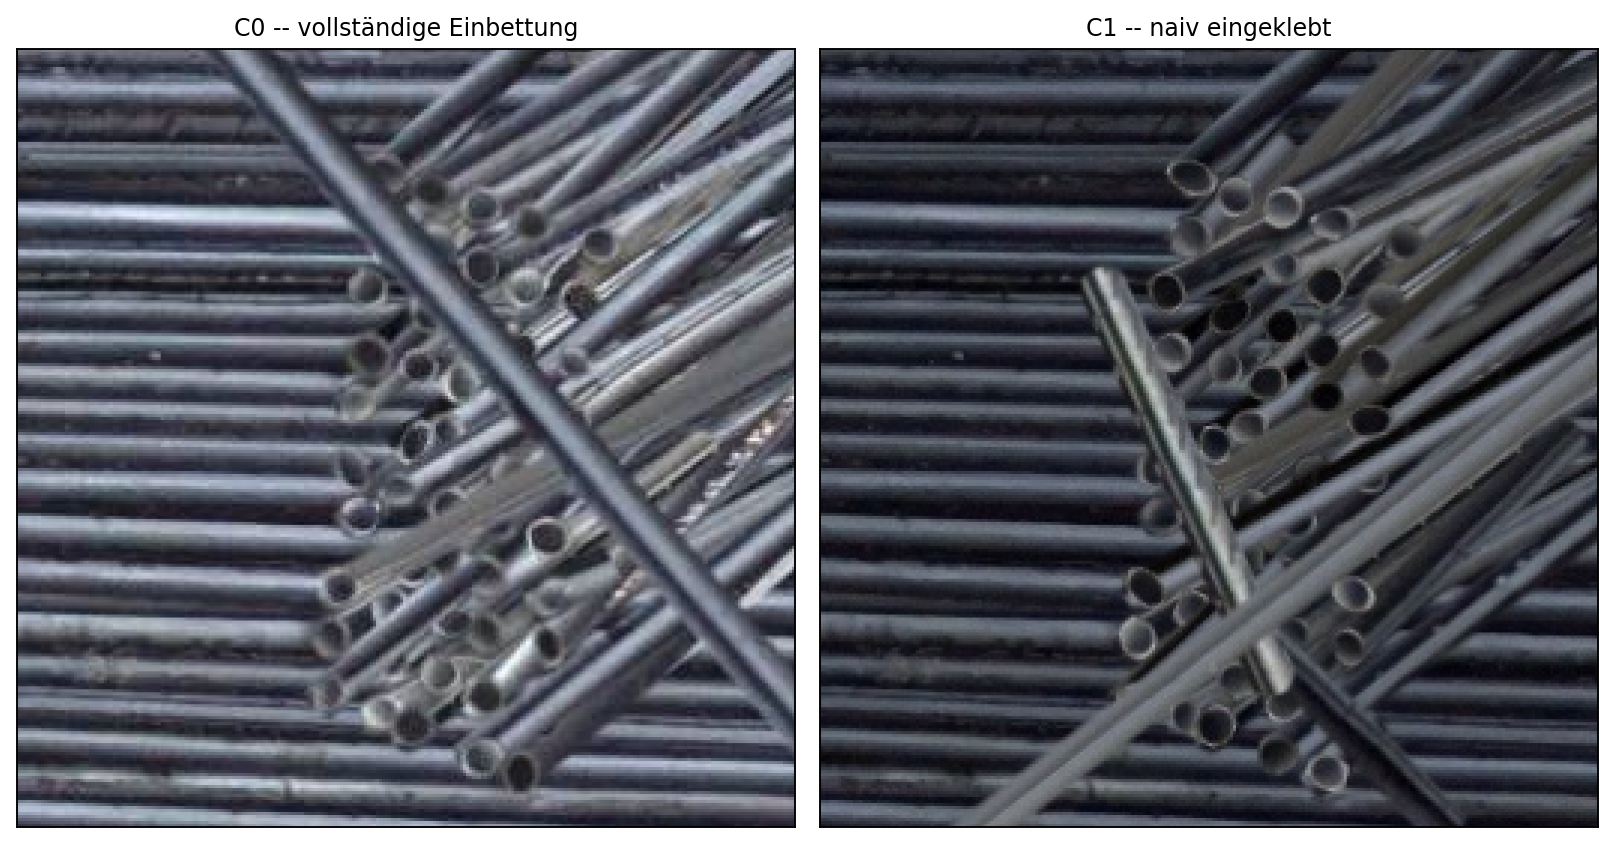
\includegraphics[width=\textwidth]{abbildungen/neu_einbettung.png}
\caption[Einbettung gegen naives Einkleben]{Je ein typischer Ausschnitt aus
beiden Armen, dreifach vergrößert. Links (C0) gehen die eingefügten Stirnflächen in
Kantenschärfe, Farbe, Rauschen und Kompression im Hintergrund auf. Rechts (C1)
stehen sie als scharf umrissene, kontrastreiche Fremdkörper auf einem
weicheren Untergrund: genau der Unterschied, den ein Faltungsnetz als
Abkürzung verwenden kann. Erzeugt mit \code{src/report\_neu.py}.}
\label{abb:einbettung}
\end{figure}

\begin{table}[htbp]
\centering
\caption[Ablation: Einbettung der eingefügten Objekte]{Ablation zur Einbettung. \code{C0} ist die vollständige Pipeline, \code{C1} dieselbe Pipeline ohne die Gegenmaßnahmen gegen die Signaturen S1--S5 und ohne Schlagschatten. \code{sval} ist der \emph{jeweils eigene} synthetische Validierungssplit des Arms und beantwortet damit die Frage, ob der Arm seine eigenen Trainingsdaten gelernt hat. Die Differenzzeile steht in Prozentpunkten, die Labelspalte absolut.}
\label{tab:ablationC}
\footnotesize
\setlength{\tabcolsep}{4pt}
\begin{tabular}{@{}lrr|rrr|rr@{}}
\toprule
\textbf{Arm} & \textbf{Labels} & \code{sval} & \multicolumn{3}{c|}{\code{test}} & \multicolumn{2}{c}{\code{val}} \\
 & & \mAPfifty{} & \mAPfifty{} & $F_1$ & $R$ & \mAPfifty{} & $F_1$ \\
\midrule
C0 Kontrolle & 68\,032 & 0{,}981 & 0{,}942 & 0{,}920 & 0{,}899 & 0{,}895 & 0{,}849 \\
C1 naiv eingeklebt & 67\,832 & 0{,}980 & 0{,}801 & 0{,}779 & 0{,}753 & 0{,}878 & 0{,}814 \\
\midrule
\emph{Differenz} & $-200$ & $-0{,}1$ & $-14{,}1$ & $-14{,}0$ & $-14{,}6$ & $-1{,}7$ & $-3{,}6$ \\
\bottomrule
\end{tabular}
\end{table}


\absatz{Ergebnis.} Ohne Einbettung ändert sich auf \code{test}, dessen
Ergebnisse in keine Entscheidung eingehen, \mAPfifty{} um
\textbf{$\zablCTestGap$\PP} (\zCOneTestMap{} gegen \zCZeroTestMap), $F_1$ um
$\zablCTestGapFf$\PP{} und der Rückruf um $\zablCTestGapRec$\PP; auf \code{val}
sind es $\zablCValGap$ und $\zablCValGapFf$\PP{} bei \mAPfifty{} und $F_1$
(Tabelle~\ref{tab:ablationC}) sowie $\zablCValGapRec$\PP{} beim Rückruf. Beide
Splits zeigen in allen drei Kennzahlen in dieselbe Richtung, aber in sehr
unterschiedlicher Größe. Einen Anhaltspunkt für die Größenordnung gibt die
Halbbreite des 95\,\%-Bootstrap-Intervalls des Referenzmodells
(Abschnitt~\ref{sec:bootstrap}): auf \code{test} rund 3\PP{}
($[\zbootTestLo;\,\zbootTestHi]$), auf \code{val} rund 4\PP{}
($[\zbootValLo;\,\zbootValHi]$). Auf \code{test} ist der Effekt rund fünfmal so
groß, auf \code{val} liegt er bei \mAPfifty{} und $F_1$ darunter; größer ist
dort nur der Rückgang des Rückrufs, dem eine höhere Precision gegenübersteht.
Ein Intervall für die Differenz der beiden Arme selbst wurde nicht berechnet,
und die Streuung des Trainings ist bei je einem Lauf unbekannt
(Abschnitt~\ref{sec:grenzen}). Belastbar ist deshalb eher die Richtung des
Effekts als seine genaue Größe.

\absatz{Synthetisch unverändert, real schlechter.} Auf seinem \emph{eigenen} synthetischen
Validierungssplit ist C1 von C0 kaum zu unterscheiden (\zCOneSval{}
gegen \zCZeroSval{} \mAPfifty, $\zablCSvalGap$\PP). Der naiv eingeklebte
Trainingssatz ist also keine schwerere Aufgabe, das Netz löst ihn ebenso gut.
Allerdings überträgt sich das Gelernte schlechter: Der Sim-to-Real-Abstand wächst auf
\code{test} von \zgapCZeroTest{} auf \zgapCOneTest\PP, also auf mehr als das
Vierfache, auf \code{val} dagegen nur von \zgapCZeroVal{} auf
\zgapCOneVal\PP.

Auf \code{test} tritt damit genau das Muster auf, das
Abschnitt~\ref{sec:hauptergebnis} als Kennzeichen von Artefaktlernen
beschrieben und beim Referenzmodell nicht gefunden hatte: synthetisch nahezu
unverändert, real deutlich schlechter. Erst dieser Vergleich gibt der Aussage
über das Referenzmodell einen Maßstab. Sein Abstand auf \code{test} beträgt
\zsimRealTest\PP{} und liegt in der Größenordnung der Kontrolle; bei C1 ist derselbe
Abstand unter sonst gleichen Bedingungen mehr als viermal so groß. Auf
\code{val} ist das Muster nur schwach ausgeprägt.

\absatz{Was der Versuch über den \emph{Mechanismus} nicht sagt.} Naheliegend
ist die Deutung, das Netz habe die Einklebespur als Abkürzung gelernt. Im
Trainingsbild trägt jedes gelabelte Objekt diese Spur und sonst kein
Bildbereich; sie ist also vollständig mit dem Label korreliert. Das Fehlermuster am
$F_1$-optimalen Betriebspunkt ist auf den beiden Splits aber verschieden. Auf
\code{test} fallen die Treffer von 80 auf 67, und zugleich steigt die Zahl der
Falsch-Positiven von 5 auf 16; die Precision sinkt von \zCZeroTestPrec{} auf
\zCOneTestPrec. Auf \code{val} fallen die Treffer von 79 auf 70, die
Falsch-Positiven dagegen von 9 auf 4, bei insgesamt \emph{weniger}
Detektionen: C1 tauscht dort Rückruf gegen Precision, und \mAPfifty{} ändert
sich kaum.

Für den Verlust kommen mehrere Erklärungen in Frage. Die eine ist die Abkürzung:
Das Netz reagiert auf die Einklebespur, die im Realbild fehlt, und liefert dort
weniger Detektionen -- das entspricht dem Muster auf \code{val}. Die andere ist eine
gewöhnliche Domänenlücke: Ohne Angleich unterscheiden sich die Trainingsobjekte
in ihrer \emph{Erscheinung} deutlich von realen Rohrenden -- schärfer,
kontrastreicher, mit dunklerer Bohrung --, und das Netz hat ein zu enges
Erscheinungsmodell gelernt, das echte Enden übersieht und an anderen Stellen
Falsch-Positive erzeugt -- das entspricht
eher dem Muster auf \code{test}. Zwei weitere Umstände können das Muster
mitprägen. Die Objektausschnitte stammen aus derselben Aufnahmeserie wie
\code{val} (Abschnitt~\ref{sec:valtest}); naiv eingeklebt tragen sie bereits
dessen Beleuchtung und Kamera, sodass der fehlende Angleich auf \code{val}
weniger ins Gewicht fällt. Und weil C1 keine JPEG-Requantisierung erhält, kann ein Teil des
Verlusts auf die Kompression der Realbilder zurückgehen statt auf die
Einbettung im engeren Sinn. Trennen kann der Versuch diese Erklärungen nicht:
Das Abschalten der Einbettung erzeugt die künstliche Kante, verfälscht die
Erscheinung des Objekts selbst und entfernt zugleich die
Kompressionsvariation. Belegt ist damit in je einem Lauf, \emph{dass} das Bündel auf dem Testbild
wirkt und dass sich sein Fehlen auf den synthetischen Daten nicht zeigt, aber
nicht, auf welchem Weg der Verlust entsteht. Einen Versuch, der das trennt,
nennt Abschnitt~\ref{sec:grenzen}.

\absatz{Konsequenz für die Pipeline.} Die Einbettungsstufen sind damit die
einzige Gruppe von Maßnahmen, deren Nutzen nicht nur begründet, sondern
gemessen ist, wenn auch nur auf dem Testbild und in je einem Lauf: Ohne sie
verlor das Modell dort rund 14 Prozentpunkte \mAPfifty; auf \code{val} bleibt
der Unterschied innerhalb der Messunsicherheit. Der eigene synthetische
Validierungssplit zeigt den Verlust nicht an.

\section{Statistische Belastbarkeit und Fehleranalyse}
\label{sec:bootstrap}

Da je Split nur \emph{ein} Bild vorliegt, ist ein gewöhnlicher Bootstrap über
Bilder nicht möglich. Verwendet wird deshalb ein räumlicher Block-Bootstrap:
Das Bild wird in $6\times6$ Kacheln zerlegt, aus denen 400-mal mit Zurücklegen
neu gezogen wird. Gezogen werden ganze Kacheln statt einzelner Objekte, weil
benachbarte Objekte nicht unabhängig sind; sie teilen Beleuchtung, Schärfe und
Verdeckungssituation \parencite{kuensch1989,efron1993}. Detektionen und
Annotationen werden vorher einmal über das ganze Bild zugeordnet wie in
Abschnitt~\ref{sec:metriken}; danach gehört jeder Treffer zur Kachel seiner
Annotation und jedes Falsch-Positiv zur Kachel seines Boxmittelpunkts. Nimmt
man jede Kachel genau einmal, ergibt sich so exakt der berichtete Wert.
Würde dagegen erst innerhalb der Kacheln zugeordnet, verlöre jedes Paar, das
auf einer Kachelgrenze liegt, seinen Treffer, und das Intervall läge
systematisch unter dem berichteten Wert. Für \mAPfifty{} ergibt sich \code{val}
$\zbootValMean \pm \zbootValStd$ mit 95\,\%-Intervall
$[\zbootValLo;\,\zbootValHi]$ (\zbootValN{} belegte Kacheln) und \code{test}
$\zbootTestMean \pm \zbootTestStd$ mit $[\zbootTestLo;\,\zbootTestHi]$
(\zbootTestN{} belegte Kacheln).

An dieser Größenordnung ist die Ablation zu messen: Kleinere
Einzeldifferenzen sind Hinweise, keine Nachweise. Zeigt eine Differenz auf
beiden Splits in dieselbe Richtung, stützt das ihre Richtung. Mehrere Metriken
desselben Bildes zählen dabei nicht als unabhängige Belege, weil \mAPfifty{},
$F_1$ und Rückruf auf denselben Detektionen beruhen. Der Auflösungseffekt von
\zswValGain\,Prozentpunkten übersteigt das Intervall dagegen um ein Vielfaches.

\begin{figure}[htbp]
\centering
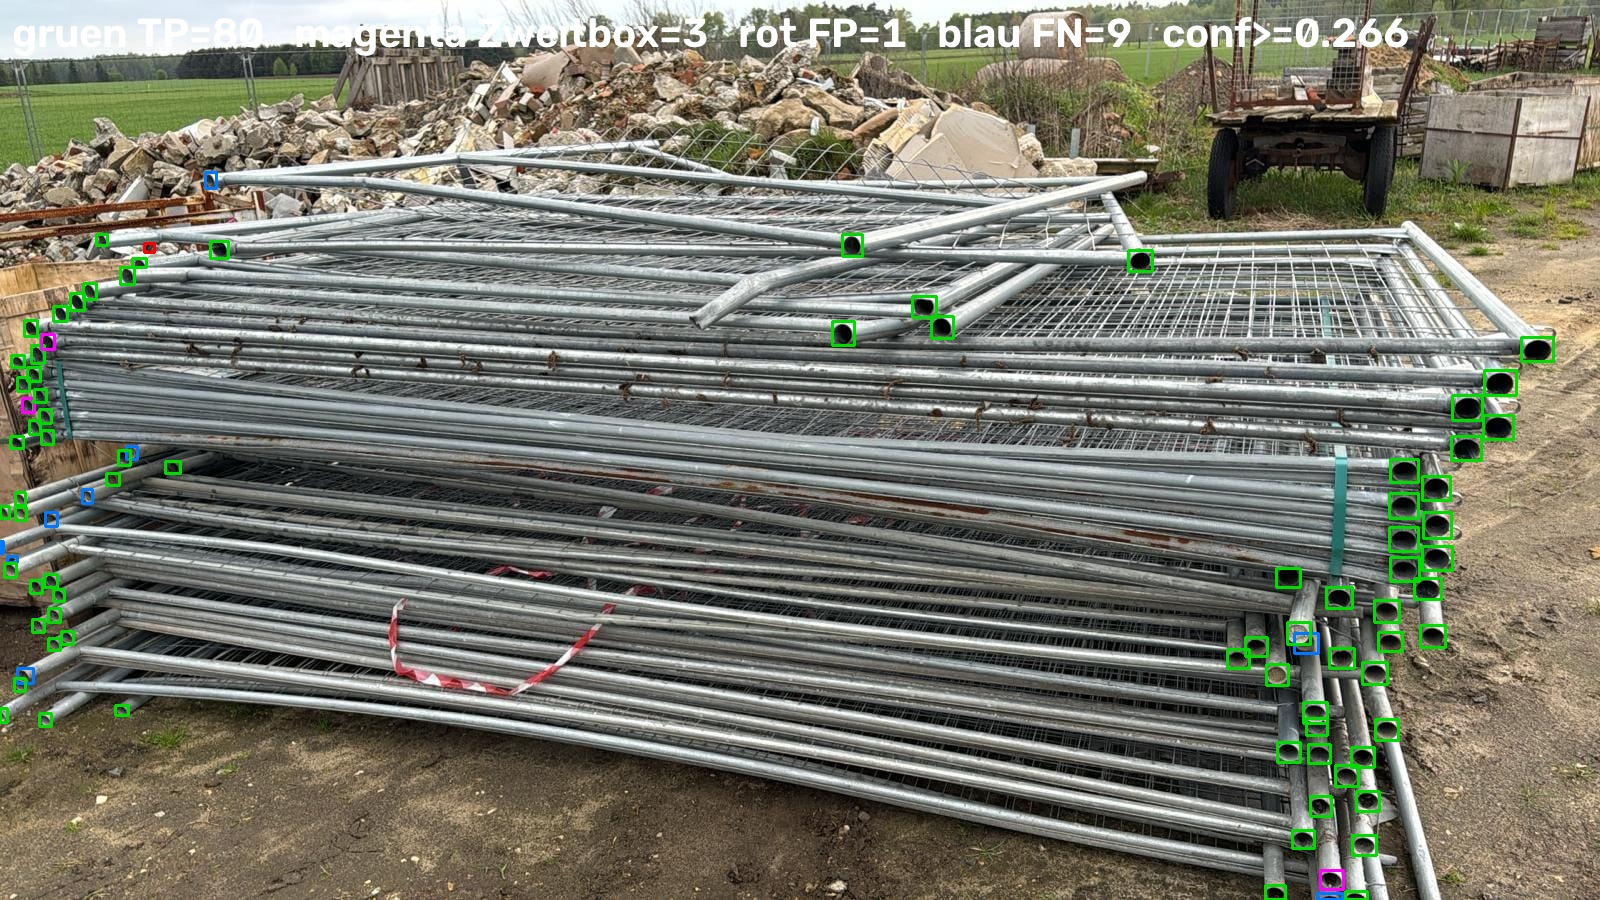
\includegraphics[width=0.93\textwidth]{abbildungen/neu_qual_test.jpg}

\vspace{4pt}
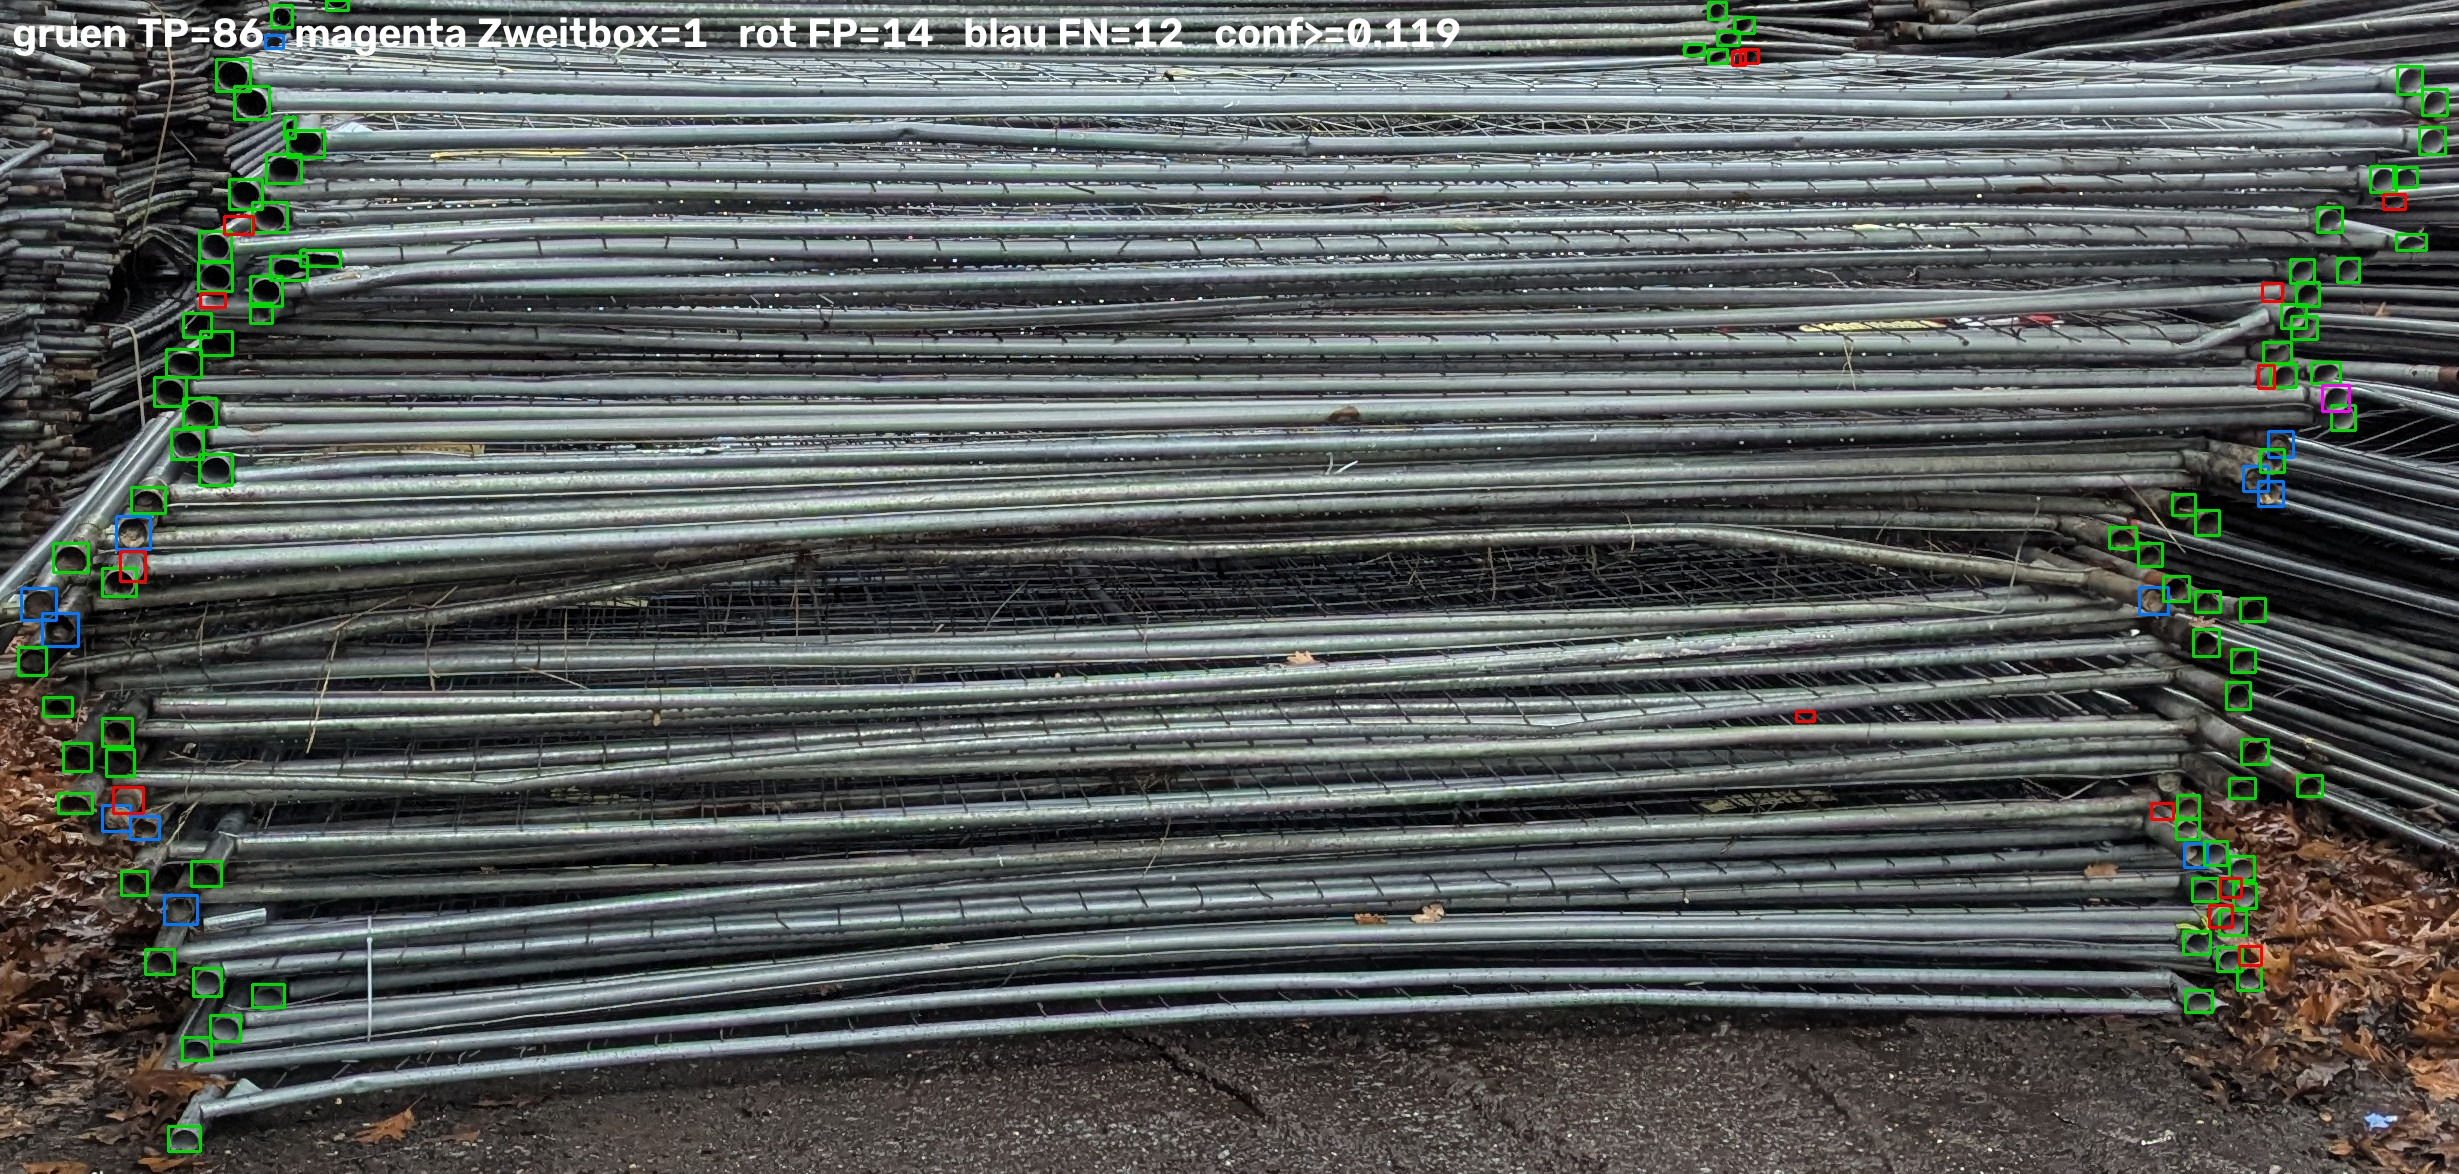
\includegraphics[width=0.93\textwidth]{abbildungen/neu_qual_val.jpg}
\caption[Qualitatives Ergebnis]{Qualitatives Ergebnis des Referenzmodells bei
der berichteten Zuordnungsschwelle $\mathrm{IoU} \geq 0{,}50$
\parencite{everingham2010,lin2014coco} und am $F_1$-optimalen Betriebspunkt.
Grün = Treffer, blau = Falsch-Negativ, magenta = Zweitbox, die eine bereits
getroffene Stirnfläche ebenfalls mit $\mathrm{IoU} \geq 0{,}50$ trifft, rot =
übrige Falsch-Positive. Zweitbox und Trefferbox sind fast deckungsgleich, die
Zweitbox verdeckt die Trefferbox deshalb im Bild.
\emph{Oben} \code{test} ($c^* = \zrefTestConf$): \zfnTest{} Falsch-Negative,
\zfpTest{} Falsch-Positive bei 89 annotierten Stirnflächen, davon
\zfpDoppelTest{} Zweitboxen. \emph{Unten} \code{val} ($c^* = \zrefValConf$):
\zfnVal{} Falsch-Negative, \zfpVal{} Falsch-Positive bei 98 annotierten
Stirnflächen, davon \zfpDoppelVal{} Zweitbox. Warum Zweitboxen entstehen und
als Fehler zählen, erklärt der Absatz \enquote{Falsch-Positive} in
Abschnitt~\ref{sec:falschpositive}. Erzeugt mit \code{src/analyse\_neu.py}.}
\label{abb:qualitativ}
\end{figure}

\absatz{Falsch-Negative.} Am $F_1$-optimalen Betriebspunkt bleiben auf
\code{test} \zfnTest{} Objekte unentdeckt, auf \code{val} \zfnVal{} (blau in
Abbildung~\ref{abb:qualitativ}). Auf
\code{test} sind \zfnKleinTest{} davon kleiner als 18\px; sie liegen
überwiegend am linken Bildrand, wo die Objekte am kleinsten sind. Daneben gibt
es einen zweiten Fehlertyp: Enden mit ungewöhnlicher Erscheinung, auf
\code{test} ein Ende ohne sichtbaren hellen Kranz, auf \code{val} vor allem
Enden, deren Bohrung mit Laub oder Rost gefüllt ist und deshalb kaum dunkler
erscheint als der Kranz. Eine helle Bohrung haben zwar drei der sechs
Quellobjekte (Abschnitt~\ref{sec:quellmaterial}), eine mit Laub oder Rost
gefüllte aber keines; hier liegt eine verbleibende Domänenlücke im
Quellmaterial selbst.

\phantomsection\absatz{Falsch-Positive.}\label{sec:falschpositive} Auf \code{test} sind sie selten: \zfpTest{} bei
\znPredTest{} Detektionen. Davon sind \zfpDoppelTest{} \emph{Zweitboxen}
(magenta in Abbildung~\ref{abb:qualitativ}): Sie
treffen ein schon erkanntes Rohrende mit $\mathrm{IoU} \geq 0{,}50$, zählen
aber als Fehler, weil die Zuordnungsregel je annotierter Fläche nur einen
Treffer zulässt \parencite{lin2014coco}, und werden nicht entfernt, weil der Kopf
NMS-frei arbeitet und der Inferenzparameter \code{iou} deshalb ohne Wirkung
bleibt (Abschnitt~\ref{sec:yolo26}); \zfpOhneTest{} überlappt keine
Annotation (rot). Auf \code{val} sind es \zfpVal{} bei \znPredVal{} Detektionen; der
$F_1$-optimale Betriebspunkt liegt dort bei der niedrigen Konfidenzschwelle
\zrefValConf. Darunter sind \zfpDoppelVal{} Zweitbox, \zfpTeilVal{} Detektionen,
die eine annotierte Stirnfläche mit einer IoU unter 0{,}50 überdecken, und
\zfpOhneVal{} ohne jede Überlappung. Eine testweise nachträgliche NMS
($\mathrm{IoU} = 0{,}7$) entfernt auf beiden Splits genau die Zweitboxen,
Treffer und Falsch-Negative bleiben gleich;
$F_1$ stiege auf \code{test} von \znmsTestFfOhne{} auf \znmsTestFfMit.
Berichtet wird ohne diesen Schritt.
Dass Zweitboxen überhaupt entstehen, liegt am Eins-zu-eins-Kopf: Im Training
ist je Stirnfläche genau eine Gitterposition positiv, jede andere soll die
Konfidenz~0 lernen (\code{tal\_topk2=1} in \code{E2ELoss},
\code{ultralytics/utils/loss.py}, Version~8.4.117). Duplikate unterdrückt er
also nur gelernt, und bei Detektoren dieser Bauart misslingt das am ehesten in
der Umgebung der konfidentesten Vorhersage, weil verschiedene Vorhersagen
desselben Objekts ähnliche Merkmale haben \parencite{wang2021defcn}.
Entsprechend stammt jede der \zzbAnzahl{} Zweitboxen aus der direkt
benachbarten Gitterzelle ihrer Trefferbox auf derselben Merkmalsebene, und beide
Boxen eines Paares sind weniger konfident als die meisten Treffer: auf
\code{test} \zzbTestConfMin{} bis \zzbTestConfMax{} bei einem Median von
\zzbTestTpConf{} über alle Treffer. Sie entstehen auch nicht erst auf den
Realbildern: Auf dem synthetischen Split \code{sval} kommen bei der Schwelle von
\code{test} \zzbSvalTestRate{} Zweitboxen auf 100 Treffer (\code{test}:
\zzbTestRate), bei der von \code{val} \zzbSvalValRate{} (\code{val}:
\zzbValRate).

\section{Ein systematischer Größenversatz der Boxen}
\label{sec:boxversatz}

Der \mAPseven{}-Wert von \zrefTestMapS{} auf \code{test} steht auffällig neben
einem \mAPfifty{} von \zrefTestMap: Das Modell \emph{findet} die meisten
Objekte, schätzt ihre Boxgröße aber systematisch zu klein.
Tabelle~\ref{tab:boxversatz} vergleicht für jede Detektion, die eindeutig auf
einem annotierten Objekt liegt ($\mathrm{IoU} > 0{,}3$), die vorhergesagte mit
der annotierten Boxgröße.

\begin{table}[htbp]
\centering
\caption[Größenversatz der Boxen]{Vergleich der vorhergesagten mit der annotierten Boxgröße. Als Boxgröße dient $\sqrt{\text{Fläche}}$, der Zentrumsversatz ist in Objektdurchmessern angegeben. \code{sval} ist der synthetische Split, dessen Labels der Generator selbst erzeugt hat.}
\label{tab:boxversatz}
\footnotesize
\begin{tabular}{@{}lrrrrr@{}}
\toprule
\textbf{Split} & \textbf{Paare} & \textbf{Objekt-\Oe{} (Median)} & \textbf{pred/GT} & \textbf{GT $-$ pred} & \textbf{Zentrumsversatz} \\
\midrule
\code{test} (real) & 88 & 17{,}9\px & 0{,}897 & $+2{,}00$\px & 0{,}051\,\Oe \\
\code{val} (real) & 97 & 26{,}8\px & 0{,}944 & $+1{,}58$\px & 0{,}056\,\Oe \\
\code{sval} (synthetisch) & 7224 & 24{,}0\px & \textbf{1{,}003} & $-0{,}08$\px & 0{,}021\,\Oe \\
\bottomrule
\end{tabular}
\end{table}


Auf dem synthetischen Split trifft das Modell die Boxgröße bis auf wenige
Promille genau (\zboxSvalRatio); auf den realen Bildern liegt sie mit
\zboxValRatio{} (\code{val}) und \zboxTestRatio{} (\code{test}) darunter. Der
Zentrumsversatz bleibt dabei mit rund \zboxTestCtr{} Objektdurchmessern im
Bereich der Annotationsgenauigkeit: Es ist ein Größen-, kein Positionsfehler.
Weil das Modell auf dem synthetischen Split die Boxgröße nahezu exakt
reproduziert, liegt die Ursache vermutlich nicht in der Boxregression, sondern
in der \emph{Labelkonvention}: Die Generatorboxen folgen der
$\alpha > 0{,}5$-Kontur der Alphamaske (Abschnitt~\ref{sec:sichtbarkeit}), die
Handannotation umschließt das Objekt großzügiger. Ausschließen lässt sich
nicht, dass auch die andere Erscheinung realer Objektkanten die vorhergesagten
Boxen verkleinert. Anforderung~A1 ist damit nur
\emph{annähernd} erfüllt; der Restversatz beträgt messbar \zboxValOff{} bis
\zboxTestOff\px.

Werden alle vorhergesagten Boxen um den gemessenen medianen Fehlbetrag von
\zsensTestGrow\px{} je Seite aufgeweitet und neu ausgewertet, so steigt
\mAPseven{} auf \code{test} von \zsensTestMapSOrig{} auf
\textbf{\zsensTestMapSNeu} und \mAPall{} von \zsensTestMapAOrig{} auf
\textbf{\zsensTestMapANeu}, während \mAPfifty{} von \zsensTestMapOrig{} auf
\zsensTestMapNeu{} leicht \emph{fällt} und das $F_1$ mit \zsensTestFfNeu{}
unverändert bleibt (Tabelle~\ref{tab:boxsens} im Anhang). Die Aufteilung ist
damit deutlich: \mAPseven{} und \mAPall{} auf \code{test} messen zu einem
erheblichen Teil eine Konventionsdifferenz und nicht die Detektionsgüte,
während \mAPfifty{} und das $F_1$ davon unberührt bleiben. Das rechtfertigt
die Festlegung aus Abschnitt~\ref{sec:metriken}, \mAPfifty{} als Leitgröße zu
verwenden.